% Copyright 2023  Ed Bueler

\documentclass[10pt,
               svgnames,
               hyperref={colorlinks,citecolor=DeepPink4,linkcolor=FireBrick,urlcolor=Maroon},
               usepdftitle=false]{beamer}

\mode<presentation>
{
  \usetheme{Madrid}

  \usecolortheme{beaver}

  \setbeamercovered{transparent}
  
  \setbeamerfont{frametitle}{size=\large}
}

\setbeamercolor*{block title}{bg=red!10}
\setbeamercolor*{block body}{bg=red!5}

\usepackage[english]{babel}
\usepackage[latin1]{inputenc}
\usepackage{times}
\usepackage[T1]{fontenc}
% Or whatever. Note that the encoding and the font should match. If T1
% does not look nice, try deleting the line with the fontenc.

\usepackage{empheq,bm,xspace,minted}
\usepackage{hyperref}
\usepackage{tikz}

% If you wish to uncover everything in a step-wise fashion, uncomment
% the following command: 
%\beamerdefaultoverlayspecification{<+->}

\newcommand{\bb}{\mathbf{b}}
\newcommand{\bc}{\mathbf{c}}
\newcommand{\bbf}{\mathbf{f}}
\newcommand{\bl}{\bm{\ell}}
\newcommand{\br}{\mathbf{r}}
\newcommand{\bs}{\mathbf{s}}
\newcommand{\bu}{\mathbf{u}}
\newcommand{\bv}{\mathbf{v}}
\newcommand{\bw}{\mathbf{w}}
\newcommand{\bx}{\mathbf{x}}
\newcommand{\by}{\mathbf{y}}
\newcommand{\bz}{\mathbf{z}}

\newcommand{\bzero}{\bm{0}}

\newcommand{\CC}{\mathbb{C}}
\newcommand{\RR}{\mathbb{R}}

\newcommand{\ddt}[1]{\ensuremath{\frac{\partial #1}{\partial t}}}
\newcommand{\ddx}[1]{\ensuremath{\frac{\partial #1}{\partial x}}}
\renewcommand{\t}[1]{\texttt{#1}}
\newcommand{\Matlab}{\textsc{Matlab}\xspace}
\newcommand{\Octave}{\textsc{Octave}\xspace}
\newcommand{\eps}{\epsilon}

\newcommand{\grad}{\nabla}
\newcommand{\Div}{\nabla \cdot}

\newcommand{\twovect}[4]{\ensuremath{{#1}_{#2} =
                            \begin{bmatrix} #3 \\ #4 \end{bmatrix}}}

\newcommand{\optimaldef}{
\begin{definition}
an algorithm for computing a function on a class of problems, which acts on floating-point data of size $N$, is \emph{optimal} if it requires
   $$O(N) \qquad \text{ or } \qquad O(N\log N) \qquad \text{ flops}$$
as $N\to\infty$
\end{definition}
}



\title{Multigrid}

\subtitle{optimal solvers for linear and nonlinear elliptic PDEs}

\author{Ed Bueler}

\institute[]{UAF Math 692 Scalable Seminar}

\date{Spring 2023}


\begin{document}
\beamertemplatenavigationsymbolsempty

\begin{frame}
  \maketitle
\end{frame}

\begin{frame}{Outline}
  \tableofcontents[hideallsubsections]
\end{frame}


\section{2 elliptic PDE problems}

\begin{frame}{a linear PDE problem}

\begin{columns}
\begin{column}{0.6\textwidth}
\begin{itemize}
\item I will consider only two PDEs today
    \begin{itemize}
    \item[1.] Poisson problem
    \item[2.] minimal surface problem
    \end{itemize}
\item both: elliptic boundary-value problems
\item recall the Laplacian $\grad^2 u =\Div(\grad u)$
    \begin{itemize}
    \item[$\circ$] in 2D: \quad $\grad^2 u = u_{xx} + u_{yy}$
    \item[$\circ$] $\grad^2$ is a negative-definite operator
    \end{itemize}
\end{itemize}
\end{column}
\begin{column}{0.4\textwidth}
\hfill 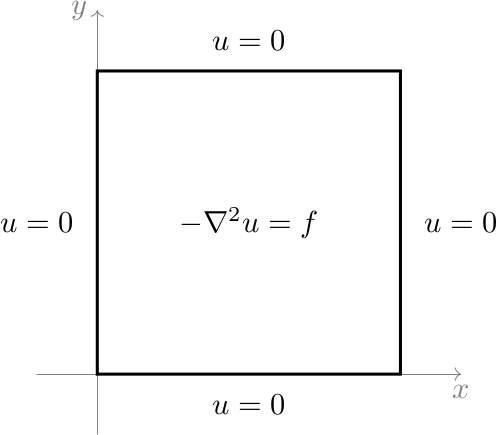
\includegraphics[width=\textwidth]{images/poisson.png}
\end{column}
\end{columns}

\bigskip
\begin{block}{1.~Poisson problem} for a given source function $f(x,y)$, find $u(x,y)$ so that
    $$-\grad^2 u = f \, \text{ on } \Omega, \qquad u\big|_{\partial \Omega} = 0$$
\end{block}
\end{frame}


\begin{frame}{a nonlinear PDE problem}

\begin{columns}
\begin{column}{0.7\textwidth}
\begin{itemize}
\item the second problem is nonlinear, but still elliptic
\item \textbf{claim 1.} the area of surface $z=v(x,y)$ over $\Omega$ is
    $$I[v] = \int_\Omega \sqrt{1 + |\grad v|^2}\,dx\,dy$$
\item \textbf{claim 2.} for given $g$, continuous along $\partial\Omega$,
    $$u = \min_{\{v \,:\, v|_{\partial \Omega} = g\}} I[v]$$
solves the boundary value problem below
\end{itemize}
\end{column}
\begin{column}{0.3\textwidth}
\hfill 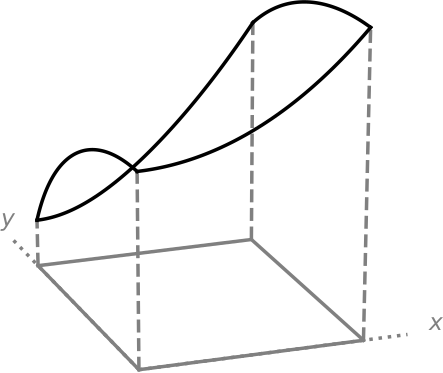
\includegraphics[width=0.75\textwidth]{images/catenary.png}

\hfill 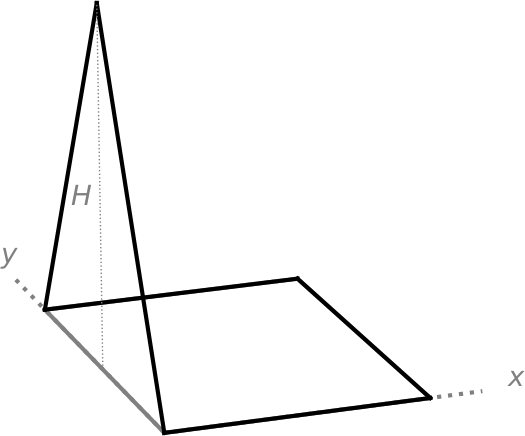
\includegraphics[width=0.75\textwidth]{images/tent.png}
\end{column}
\end{columns}

\medskip
\begin{block}{2.~minimal surface problem} for given boundary function (wire frame) $g(x,y)$, find $u(x,y)$ so that
    $$-\Div \left(\frac{\grad u}{\sqrt{1 + |\grad u|^2}}\right) = 0 \, \text{ on } \Omega, \qquad u\big|_{\partial \Omega} = g$$
\end{block}
\end{frame}


\begin{frame}{finite difference discretization}
\begin{columns}
\begin{column}{0.7\textwidth}
\begin{itemize}
\item PDEs are infinite-dimensional problems!
\item discretization yields finite systems of equations
\item for example, finite differences (FD):
    $$f''(x) = \frac{f(x+h) - 2 f(x) + f(x-h)}{h^2} + O(h^2)$$
\item our 2D test problem will have $\Omega = (0,1) \times (0,1)$
\item define spacings \strut $h_x=\frac{1}{m_x-1}$, $h_y=\frac{1}{m_y-1}$
\item grid points are $(x_i,y_j) = (ih_x,jh_y)$ for $i=0,\dots,m_x-1$ and $j=0,\dots,m_y-1$
\item 5-point stencil for the Laplacian:
{\small
$$\grad^2 u(x_i,y_j) \approx \frac{U_{i-1,j} - 2 U_{ij} + U_{i+1,j}}{h_x^2} + \frac{U_{i,j-1} - 2 U_{ij} + U_{i,j+1}}{h_y^2}$$
}
\end{itemize}
\end{column}
\begin{column}{0.3\textwidth}
\hfill 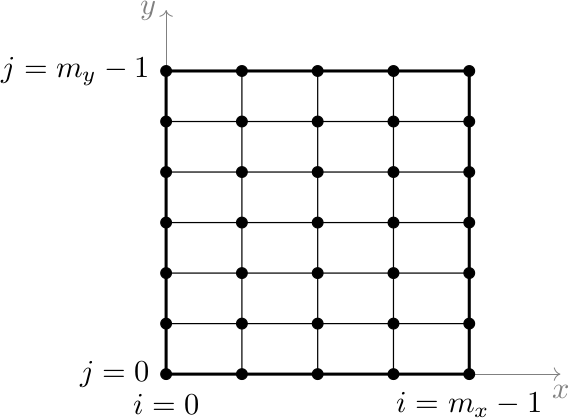
\includegraphics[width=\textwidth]{images/gridindexing.png}

\vspace{15mm}
\hfill 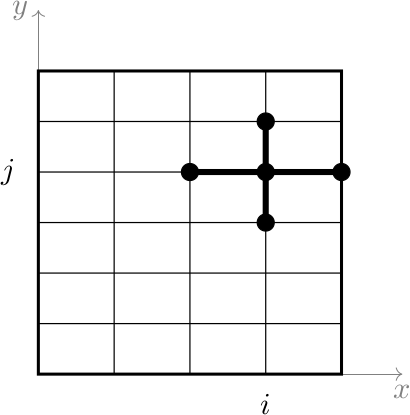
\includegraphics[width=0.7\textwidth]{images/gridstencil.png}
\end{column}
\end{columns}
\end{frame}


% next slide spy plots from Matlab (NOT OCTAVE):
%   m=5; spy(delsq(numgrid('S',m)),'k'), axis off,  print -dpdf lapspy5.pdf
%   m=8; spy(delsq(numgrid('S',m)),8,'k'), axis off,  print -dpdf lapspy8.pdf
% then pdfcrop

\begin{frame}{PDE $\implies$ linear system $A\bu=\bb$}
\begin{columns}
\begin{column}{0.73\textwidth}
\begin{itemize}
\item consider the 2D Poisson equation $-\grad^2 u = f$
\item if we choose $m_x,m_y$ subintervals in the two directions, then there are $N=m_x m_y$ total unknowns on the grid
\item the PDE becomes a linear system for $\bu \in \RR^N$:
	$$A\, \bu = \bb$$

	\begin{itemize}
	\item[$\circ$] unknowns $\{U_{ij}\}$ are globally ordered $k=0,1,\dots,N-1$ (upper right)
	\item[$\circ$] $A \in \RR^{N\times N}$ is symmetric positive definite
	\item[$\circ$] we \textbf{keep} the boundary values in the linear system
	\item[$\circ$] $\bb \in \RR^N$ has entries $b_k = f(x_i,y_j)$
	\end{itemize}
\item for $m=5$: 9 \textbf{non-trivial} equations (middle right)
\item for $m=8$: 36 \textbf{non-trivial} equations (lower right)
\end{itemize}
\end{column}
\begin{column}{0.27\textwidth}
\hfill 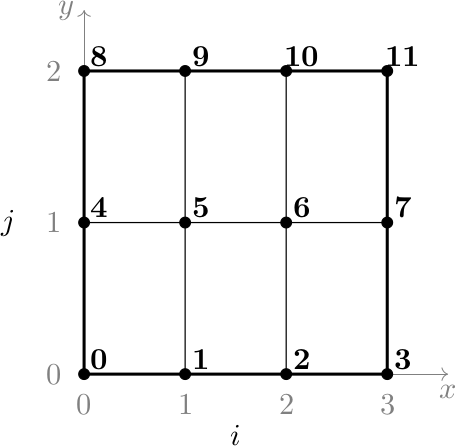
\includegraphics[width=0.9\textwidth]{images/gridordering.png}

\bigskip\medskip
\hfill 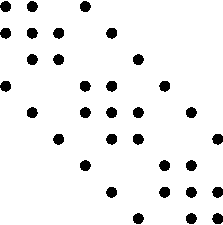
\includegraphics[width=0.5\textwidth]{images/lapspy5.pdf}

\bigskip
\hfill 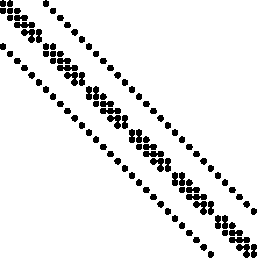
\includegraphics[width=0.7\textwidth]{images/lapspy8.pdf}

\end{column}
\end{columns}
\end{frame}


\begin{frame}{goal: solve $A\bu=\bb$ in $O(N)$ work}
\begin{itemize}
\item the linear system $A\bu=\bb$ can be set-up using  $6N$ memory locations
	\begin{itemize}
	\item[$\circ$] $A$ has 5 nonzero entries per row
	\end{itemize}
\item $A$ is banded, with bandwidth $\approx \sqrt{N}=m$
	\begin{itemize}
	\item[$\circ$] banded Gaussian elimination should solve in $O(N^2)$
	\end{itemize}
\item how to solve $A\bu=\bb$ in $O(N)$ work and time?

\bigskip
\item<2> simpler question first:

\medskip
\qquad what operations using \emph{this} $A$ are obviously $O(N)$?
\end{itemize}
\end{frame}


\section{regarding simple iterations}

\begin{frame}{cheap $O(N)$ operation: residual}
\begin{itemize}
\item we can compute $A\bv$, for any vector $\bv$, in $O(N)$ flops
\item also the residual is $O(N)$

\begin{definition} given $\bv \in\RR^N$, the \emph{residual} for the linear system $A\bu=\bb$ is
	$$\br(\bv) = \bb - A\bv$$
\end{definition}

\item notice: $A\bu = \bb \quad \iff \quad \br(\bu) = 0$
\end{itemize}
\end{frame}


\begin{frame}{cheap $O(N)$ operations: \emph{certain} simple iterations}

\begin{definition} for the linear system $A\bu=\bb$, an invertible matrix $M\in \RR^{N\times N}$, and scalar $\alpha$,
    $$\bv_{k+1} = \bv_k + \alpha M^{-1} \left(\bb - A \bv_k\right)$$
is called \emph{simple iteration}
\end{definition}

\bigskip
\begin{itemize}
\item a simple iteration is $O(N)$ \dots \emph{if} $M$ is the right kind of matrix
\item \emph{Richardson} iteration is when $M=I$; clearly $O(N)$
\end{itemize}

\bigskip
\begin{definition} a matrix or linear map $M$ is an \emph{optimal preconditioner} if solving $M\bz=\bc$ requires $O(N)$ work
\end{definition}

\bigskip
\begin{itemize}
\item warning: a preconditioner $M$ can be optimal without being a good preconditioner!
\end{itemize}
\end{frame}


\begin{frame}{$O(N)$ simple iterations: Jacobi and Gauss-Seidel}
\begin{itemize}
\item suppose we split into diagonal and triangular parts:
	$$A=D + L + U$$
\only<1>{
\item the linear system can be rearranged using the splitting:
\begin{align*}
A\bu=\bb \quad &\iff \quad D \bu = \bb - (L+U) \bu \\
               &\iff \quad \bu = \bu + D^{-1} (\bb - A \bu)
\end{align*}
\item solving $D\bz = \bc$ is $O(N)$
\begin{definition}
each \emph{Jacobi iteration}, a simple iteration, is $O(N)$:
	$$\bv_{k+1} = \bv_k + D^{-1} (\bb - A \bv_k)$$
\end{definition}
}
\only<2>{
\item the linear system can be rearranged using the splitting:
\begin{align*}
A\bu=\bb \quad &\iff \quad (D+L) \bu = \bb - U \bu \\
               &\iff \quad \bu = \bu + (D+L)^{-1} (\bb - A \bu)
\end{align*}
\item for $A$ from the Poisson equation, solving $(D+L)\bz=\bc$ is $O(N)$

\begin{definition}
each \emph{Gauss-Seidel iteration}, a simple iteration, is $O(N)$:
	$$\bv_{k+1} = \bv_k + (D+L)^{-1} (\bb - A \bv_k)$$
\end{definition}
}
\end{itemize}
\end{frame}

\begin{frame}{solving effect of Jacobi and Gauss-Seidel iterations}
\begin{itemize}
\item FIXME not good solvers ... Figure 6.1

\hfill 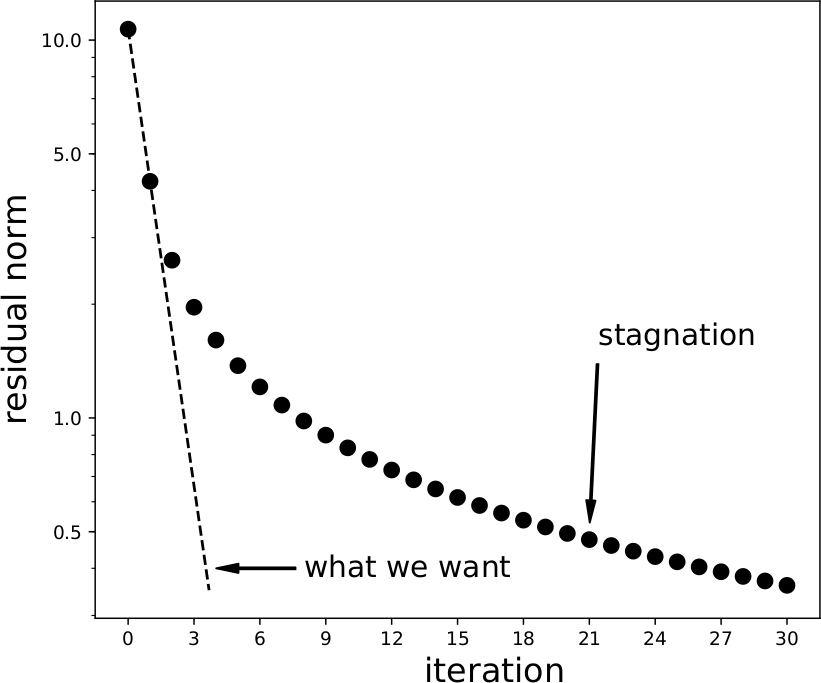
\includegraphics[width=0.45\textwidth]{images/stagnation.png}

\item an inventor of multigrid, Achi Brandt, famously says:
\begin{quotation}
Stalling numerical processes must be wrong.

Whenever the computer grinds very hard for

small or slow effect, there must be a better

way to achieve the same goal.
\end{quotation}

\vspace{-19mm}
\hfill 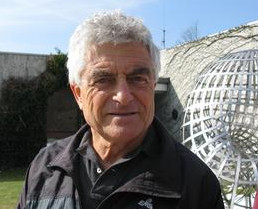
\includegraphics[width=0.18\textwidth]{images/abrandt.jpg}
\end{itemize}
\end{frame}



\begin{frame}{\emph{smoothing} effect of Jacobi and Gauss-Seidel iterations}
\begin{itemize}
\item FIXME but smoothers Figure 6.2, 6.3

\only<1>{
\hfill 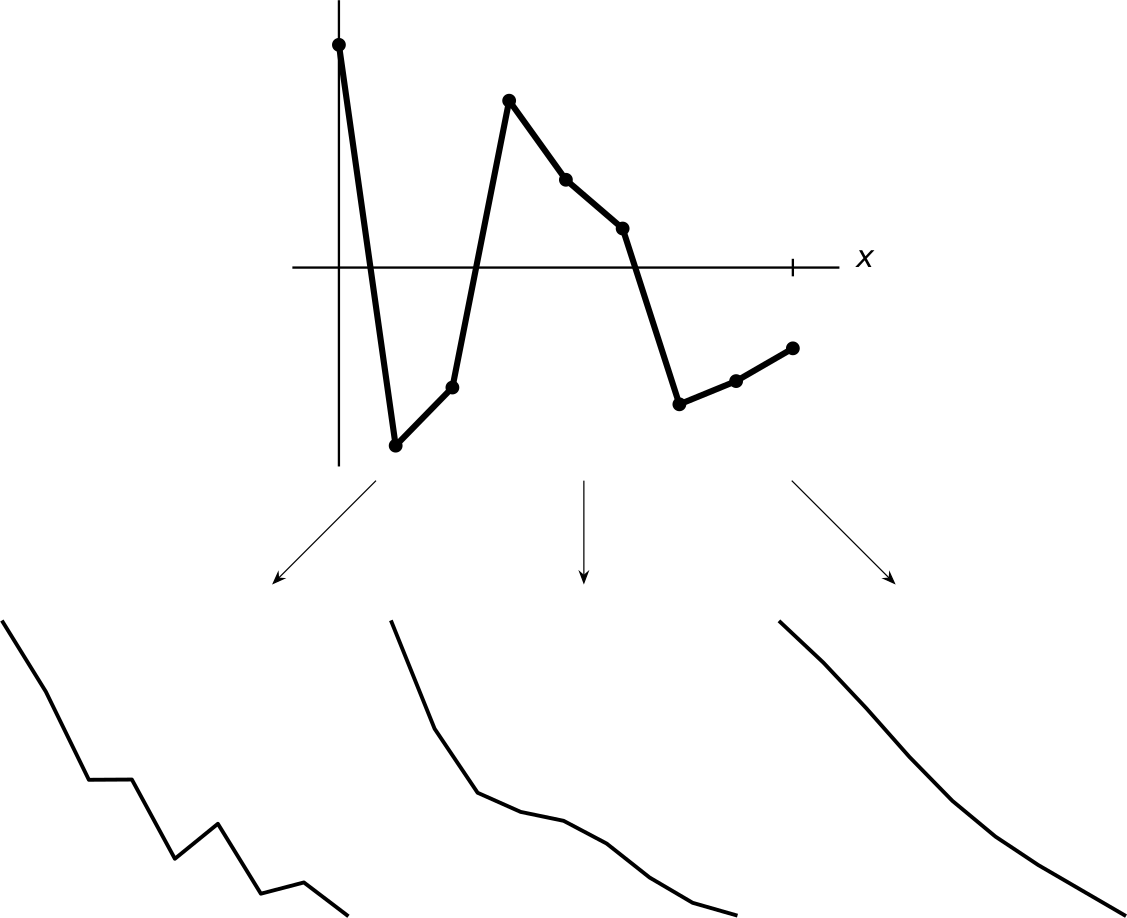
\includegraphics[height=0.75\textheight]{images/smoothing-space.png}
}
\only<2>{
\hfill 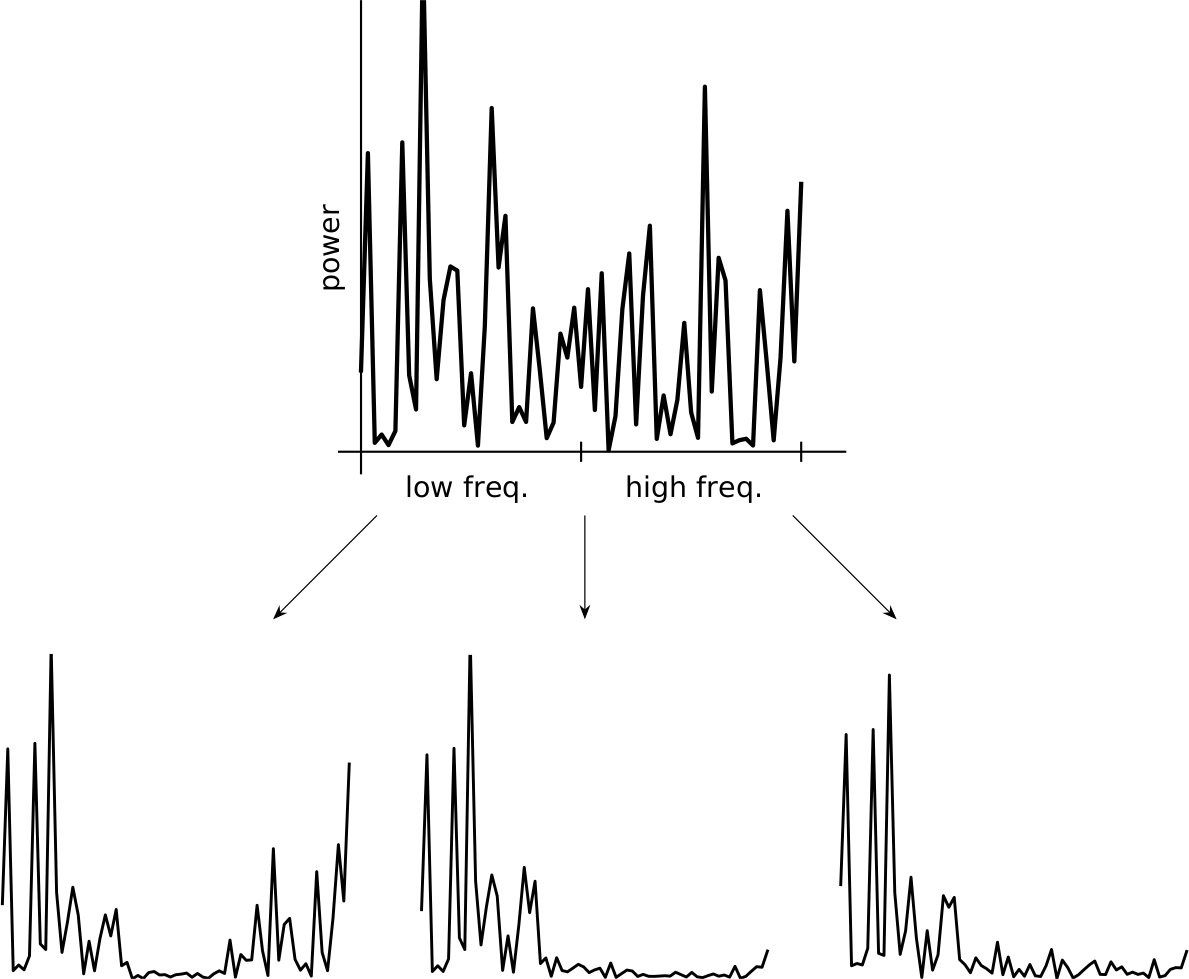
\includegraphics[height=0.75\textheight]{images/smoothing-freq.png}
}
\end{itemize}
\end{frame}


\section{the coarse-grid correction}

\begin{frame}{x}
\begin{itemize}
\item x
\end{itemize}
\end{frame}



\section{the 2-grid and V cycles}

\begin{frame}{x}
\begin{columns}
\begin{column}{0.8\textwidth}
\begin{itemize}
\item x
\end{itemize}
\end{column}
\begin{column}{0.17\textwidth}
\hfill 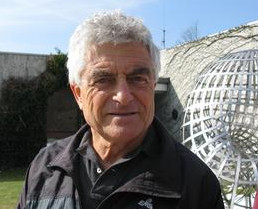
\includegraphics[width=\textwidth]{images/abrandt.jpg}
\end{column}
\end{columns}
\end{frame}



\section{multigrid as an optimal solver}

\begin{frame}{x}
\begin{itemize}
\item x
\end{itemize}
\end{frame}

\begin{frame}{nonlinear F-cycle solvers}
\begin{itemize}
\item x

\hfill 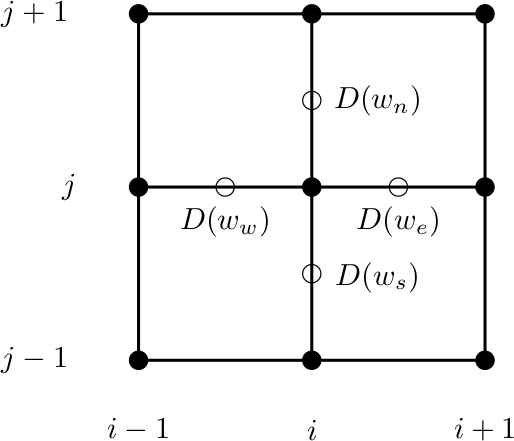
\includegraphics[width=0.3\textwidth]{images/msboxstencil.png}
\end{itemize}
\end{frame}


\begin{frame}[fragile]
\frametitle{\texttt{matvec}}
\begin{itemize}
\item y
\end{itemize}
\begin{center}
\begin{minipage}{0.7\textwidth}
\begin{minted}[fontsize=\small]{python}
def matvec(A,x):
    from numpy import zeros, shape
    [m,n] = shape(A)
    z = zeros((m,1))
    for i in range(m):
        s = 0.0
        for j in range(n):
            s += A[i][j] * x[j]
        z[i] = s
    return z
\end{minted}
\end{minipage}
\end{center}
\end{frame}


\begin{frame}{references}

\begin{columns}
\begin{column}{0.8\textwidth}
\begin{itemize}
{\small
\item[] \textbf{A.~Brandt (1977)}. \emph{Multi-level adaptive solutions to boundary-value problems}, Mathematics of Computation 31 (138), 333--390
    \begin{itemize}
    \item[$\circ$] the guru of multigrid should be better known
    \end{itemize}
\item[] \textbf{W.~Briggs, V.~E.~Henson, \& S.~McCormick (2000)}.  \emph{A Multigrid Tutorial}, 2nd ed., SIAM Press, Philadelphia
    \begin{itemize}
    \item[$\circ$] straightforward introduction
    \end{itemize}
\item[] \textbf{E.~Bueler (2021)}. \emph{PETSc for Partial Differential Equations}, SIAM Press, Philadelphia
    \begin{itemize}
    \item[$\circ$] Krylov methods, preconditioners, many multigrid solver examples
    \end{itemize}
\item[] \textbf{H.~Elman, D.~Silvester, \& A.~Wathen (2014)}. \emph{Finite Elements and Fast Iterative Solvers: With Applications to Incompressible Fluid Dynamics}, 2nd ed., Oxford U.~Press
    \begin{itemize}
    \item[$\circ$] multigrid in the fluids context
    \end{itemize}
\item[] \textbf{U.~Trottenberg, C.~Oosterlee, \& A. Schuller (2001)}.  \emph{Multigrid}, Elsevier, Oxford
    \begin{itemize}
    \item[$\circ$] a comprehensive view
    \end{itemize}
}
\end{itemize}
\end{column}
\begin{column}{0.17\textwidth}
\hfill 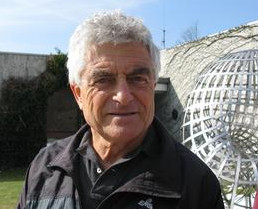
\includegraphics[width=\textwidth]{images/abrandt.jpg}

\hfill {\scriptsize \emph{Achi Brandt}}

\vspace{10mm}
\hfill 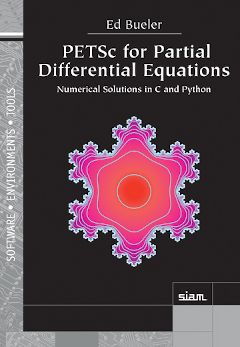
\includegraphics[width=0.9\textwidth]{images/bueler.jpg}

\vspace{20mm}
\end{column}
\end{columns}
\end{frame}

\end{document}
